% Quantitative white-beam XRF mapping on BM32 -- processing chain
% Compile with:  tectonic xrf_quantification.tex   (or latexmk -xelatex / -pdf)
% All numbers derived from the data are macros \r... defined in results_macros.tex,
% generated by make_figures.py -> results.json -> make_macros.py.
\documentclass[11pt,a4paper]{article}
\usepackage[margin=2.4cm]{geometry}
\usepackage{iftex}
\ifPDFTeX
  \usepackage[T1]{fontenc}\usepackage[utf8]{inputenc}\usepackage{lmodern}
\fi
\usepackage{amsmath,amssymb}
\usepackage{graphicx}
\usepackage{booktabs,tabularx,multirow}
\usepackage[separate-uncertainty=true,range-phrase=--]{siunitx}
\usepackage{xcolor}
\usepackage[font=small,labelfont=bf]{caption}
\usepackage[numbers,sort&compress]{natbib}
\usepackage{microtype}
\usepackage[colorlinks=true,linkcolor=blue!50!black,citecolor=green!35!black,urlcolor=blue!60!black]{hyperref}
\usepackage{enumitem}

% generated by make_macros.py from results.json -- do not edit
\newcommand{\rNPix}{6561}
\newcommand{\rNSlow}{81}
\newcommand{\rNFast}{81}
\newcommand{\rStepUm}{0.25}
\newcommand{\rCountTime}{1}
\newcommand{\rCountsPerPixel}{\num{7.32e4}}
\newcommand{\rTotalCounts}{\num{4.80e8}}
\newcommand{\rIcrMin}{86.8}
\newcommand{\rIcrMean}{96.6}
\newcommand{\rIcrMax}{105.3}
\newcommand{\rOcrMean}{72.7}
\newcommand{\rDeadMin}{0.230}
\newcommand{\rDeadMed}{0.250}
\newcommand{\rDeadMax}{0.259}
\newcommand{\rLiveMin}{0.746}
\newcommand{\rLiveMax}{0.776}
\newcommand{\rRealTime}{1.008}
\newcommand{\rMonSpread}{17.9}
\newcommand{\rScanHours}{2.68}
\newcommand{\rScanSec}{9645}
\newcommand{\rRoiLo}{292}
\newcommand{\rRoiHi}{1261}
\newcommand{\rCalGain}{10.032}
\newcommand{\rCalOffset}{-31.263}
\newcommand{\rRateMonCorr}{0.983}
\newcommand{\rRateRowSpread}{4.33}
\newcommand{\rRateMonRowSpread}{1.14}
\newcommand{\rGaRowSpread}{1.02}
\newcommand{\rRefillARow}{3}
\newcommand{\rRefillACol}{8}
\newcommand{\rRefillATime}{470}
\newcommand{\rRefillAMon}{17.9}
\newcommand{\rRefillARate}{15.4}
\newcommand{\rRefillAGa}{-1.85}
\newcommand{\rRefillAAs}{-1.79}
\newcommand{\rRefillARatio}{-0.06}
\newcommand{\rRefillBRow}{33}
\newcommand{\rRefillBCol}{12}
\newcommand{\rRefillBTime}{4075}
\newcommand{\rRefillBMon}{17.6}
\newcommand{\rRefillBRate}{15.1}
\newcommand{\rRefillBGa}{-1.83}
\newcommand{\rRefillBAs}{-1.79}
\newcommand{\rRefillBRatio}{-0.04}
\newcommand{\rRefillCRow}{63}
\newcommand{\rRefillCCol}{54}
\newcommand{\rRefillCTime}{7671}
\newcommand{\rRefillCMon}{18.0}
\newcommand{\rRefillCRate}{14.4}
\newcommand{\rRefillCGa}{-2.73}
\newcommand{\rRefillCAs}{-2.62}
\newcommand{\rRefillCRatio}{-0.11}
\newcommand{\rEc}{20.86}
\newcommand{\rBandTenLo}{8.6}
\newcommand{\rBandTenHi}{29.1}
\newcommand{\rBandOneLo}{7.2}
\newcommand{\rBandOneHi}{30.9}
\newcommand{\rPeakBW}{19.8}
\newcommand{\rPeakKeV}{16.6}
\newcommand{\rkBW}{1.142}
\newcommand{\rkKeV}{1.054}
\newcommand{\rkJacobianBias}{8.4}
\newcommand{\rEffIn}{0.0356}
\newcommand{\rEffGa}{0.845}
\newcommand{\rEffAs}{0.853}
\newcommand{\rEffAsKb}{0.819}
\newcommand{\rEffInPerCm}{0.847}
\newcommand{\rEffGaPerCm}{0.992}
\newcommand{\rEffInLowP}{1.079}
\newcommand{\rEscGa}{0.126}
\newcommand{\rEscIn}{1.08}
\newcommand{\rEscMax}{1.76}
\newcommand{\rEscMaxE}{1.88}
\newcommand{\rTau}{0.115}
\newcommand{\rTauNs}{115}
\newcommand{\rTauErr}{0.0002}
\newcommand{\rTauChiWith}{1295}
\newcommand{\rTauChiWithout}{1429}
\newcommand{\rPairProb}{1.1}
\newcommand{\rChiScalar}{1611}
\newcommand{\rInLbScalar}{0.446}
\newcommand{\rInLbiiiScalar}{0.110}
\newcommand{\rInLbivScalar}{0.159}
\newcommand{\rAsKbScalar}{0.1467}
\newcommand{\rAsKaiiScalar}{0.5153}
\newcommand{\rChiWhite}{1618}
\newcommand{\rInLbWhite}{0.475}
\newcommand{\rInLbiiiWhite}{0.110}
\newcommand{\rInLbivWhite}{0.124}
\newcommand{\rAsKbWhite}{0.1467}
\newcommand{\rAsKaiiWhite}{0.5153}
\newcommand{\rChiWhiteEff}{1648}
\newcommand{\rInLbWhiteEff}{0.803}
\newcommand{\rInLbiiiWhiteEff}{0.297}
\newcommand{\rInLbivWhiteEff}{0.254}
\newcommand{\rAsKbWhiteEff}{0.1408}
\newcommand{\rAsKaiiWhiteEff}{0.5156}
\newcommand{\rChiMatrix}{1531}
\newcommand{\rInLbMatrix}{0.856}
\newcommand{\rInLbiiiMatrix}{0.335}
\newcommand{\rInLbivMatrix}{0.273}
\newcommand{\rAsKbMatrix}{0.1436}
\newcommand{\rAsKaiiMatrix}{0.5152}
\newcommand{\rNiNoEsc}{30.4}
\newcommand{\rNiEsc}{12.6}
\newcommand{\rChiNoEsc}{1493}
\newcommand{\rChiEsc}{1525}
\newcommand{\rChi}{1525}
\newcommand{\rNChan}{969}
\newcommand{\rNFree}{14}
\newcommand{\rNLines}{39}
\newcommand{\rNGroups}{7}
\newcommand{\rNoise}{28.6}
\newcommand{\rFano}{0.160}
\newcommand{\rFanoW}{0.168}
\newcommand{\rGamma}{11.9}
\newcommand{\rFwhmMn}{157}
\newcommand{\rFwhmGa}{190}
\newcommand{\rResidRms}{0.42}
\newcommand{\rAreaIn}{89.44}
\newcommand{\rAreaErrIn}{0.11}
\newcommand{\rSnrIn}{8.0}
\newcommand{\rAreaGa}{16074}
\newcommand{\rAreaErrGa}{1.4}
\newcommand{\rSnrGa}{138}
\newcommand{\rAreaAs}{33591}
\newcommand{\rAreaErrAs}{2.1}
\newcommand{\rSnrAs}{204}
\newcommand{\rAreaCu}{10.77}
\newcommand{\rAreaErrCu}{0.08}
\newcommand{\rSnrCu}{2.4}
\newcommand{\rAreaNi}{12.58}
\newcommand{\rAreaErrNi}{0.09}
\newcommand{\rSnrNi}{1.5}
\newcommand{\rAreaCa}{37.44}
\newcommand{\rAreaErrCa}{0.11}
\newcommand{\rSnrCa}{3.4}
\newcommand{\rAreaAr}{10.18}
\newcommand{\rAreaErrAr}{0.07}
\newcommand{\rSnrAr}{2.4}
\newcommand{\rxGa}{0.4825}
\newcommand{\rxIn}{0.835}
\newcommand{\rClosure}{1.317}
\newcommand{\rIter}{4}
\newcommand{\rkGa}{1.0083}
\newcommand{\rkIn}{313.5}
\newcommand{\rSFGa}{5.65}
\newcommand{\rSFIn}{7.50}
\newcommand{\rSFAs}{0.027}
\newcommand{\rAbsGa}{0.865}
\newcommand{\rAbsAs}{0.871}
\newcommand{\rAbsIn}{0.578}
\newcommand{\rCapInFrac}{6.1}
\newcommand{\rCapInSF}{5.9}
\newcommand{\rCapTIn}{0.980}
\newcommand{\rCapTGa}{0.995}
\newcommand{\rCapTAs}{0.996}
\newcommand{\rSFGaAsKLiii}{3.29}
\newcommand{\rSFGaAsKLii}{1.71}
\newcommand{\rSFGaAsKMiii}{0.40}
\newcommand{\rSFInAsKLiii}{2.63}
\newcommand{\rSFInGaKLiii}{1.72}
\newcommand{\rxGaNoCap}{0.4826}
\newcommand{\rxInNoCap}{0.873}
\newcommand{\rClosureNoCap}{1.355}
\newcommand{\rxGaNoMatrix}{0.5056}
\newcommand{\rxInNoMatrix}{0.652}
\newcommand{\rClosureNoMatrix}{1.158}
\newcommand{\rCapScanZero}{1.355}
\newcommand{\rCapScanOne}{1.281}
\newcommand{\rCapScanTwo}{1.211}
\newcommand{\rCapScanThree}{1.145}
\newcommand{\rCapScanFour}{1.083}
\newcommand{\rCapScanFive}{1.024}
\newcommand{\rSensitivityRows}{%
nominal & 0.4825 & \num{+0.0} & 0.835 & 1.317 \\
air 18 cm & 0.4731 & \num{-2.0} & 0.600 & 1.073 \\
air 22 cm & 0.4922 & \num{+2.0} & 1.157 & 1.649 \\
take-off 30\si{\degree} & 0.4850 & \num{+0.5} & 0.915 & 1.400 \\
take-off 50\si{\degree} & 0.4812 & \num{-0.3} & 0.790 & 1.271 \\
film 1.52 \si{\micro\metre} & 0.4846 & \num{+0.4} & 0.778 & 1.262 \\
film 2.28 \si{\micro\metre} & 0.4811 & \num{-0.3} & 0.890 & 1.371 \\
cap 30 nm & 0.4825 & \num{+0.0} & 0.850 & 1.332 \\
cap 70 nm & 0.4825 & \num{+0.0} & 0.820 & 1.303 \\
no cap & 0.4826 & \num{+0.0} & 0.873 & 1.355 \\
990 hPa & 0.4803 & \num{-0.5} & 0.774 & 1.255 \\}
\newcommand{\rxGaMin}{0.473}
\newcommand{\rxGaMax}{0.492}
\newcommand{\rClosureMin}{1.07}
\newcommand{\rClosureMax}{1.65}
\newcommand{\rClosureAirLo}{1.07}
\newcommand{\rClosureAirHi}{1.65}
\newcommand{\rWinLo}{8842}
\newcommand{\rWinHi}{9661}
\newcommand{\rStepRow}{25}
\newcommand{\rNCentroidSteps}{0}
\newcommand{\rWidthErr}{0.06}
\newcommand{\rWidthBefore}{87.6}
\newcommand{\rWidthAfter}{94.9}
\newcommand{\rWidthJump}{8.4}
\newcommand{\rCentroidRange}{1.9}
\newcommand{\rFwhmSegA}{182.2}
\newcommand{\rFwhmSegB}{194.1}
\newcommand{\rGammaSegA}{10.0}
\newcommand{\rGammaSegB}{12.5}
\newcommand{\rChiSegA}{410}
\newcommand{\rChiSegB}{1139}
\newcommand{\rInvariance}{\num{6.9e-15}}
\newcommand{\rChangePix}{6}
\newcommand{\rChangePixPrev}{5}
\newcommand{\rChangeTime}{3038}
\newcommand{\rWcFirst}{-8.5}
\newcommand{\rWcBeforeChange}{-6.9}
\newcommand{\rWcAtChange}{-1.4}
\newcommand{\rRoiRatioBefore}{0.4639}
\newcommand{\rRoiRatioAfter}{0.4639}
\newcommand{\rIcrBefore}{97.7}
\newcommand{\rIcrAfter}{96.1}
\newcommand{\rModeRows}{%
\texttt{none} & \num{-1.16} & 1.16 & 1.079 & 0.96--1.26 \\
\texttt{segments} & \num{+0.14} & 1.03 & 0.999 & 0.89--1.11 \\
\texttt{linear} & \num{-0.19} & 1.03 & 1.009 & 0.91--1.12 \\
\texttt{both} & \num{+0.15} & 1.03 & 0.998 & 0.89--1.11 \\}
\newcommand{\rStepNone}{-1.16}
\newcommand{\rSpreadNone}{1.16}
\newcommand{\rChiMapNone}{1.079}
\newcommand{\rStepSeg}{0.14}
\newcommand{\rSpreadSeg}{1.03}
\newcommand{\rChiMapSeg}{0.999}
\newcommand{\rStepLin}{-0.19}
\newcommand{\rSpreadLin}{1.03}
\newcommand{\rChiMapLin}{1.009}
\newcommand{\rStepBoth}{0.15}
\newcommand{\rSpreadBoth}{1.03}
\newcommand{\rChiMapBoth}{0.998}
\newcommand{\rxMed}{0.4817}
\newcommand{\rxSpread}{0.0050}
\newcommand{\rxStat}{0.0042}
\newcommand{\rxExcess}{0.0026}
\newcommand{\rxNoneMed}{0.4811}
\newcommand{\rxNoneSpread}{0.0056}
\newcommand{\rxExcessNone}{0.0035}
\newcommand{\rCurveAbsGaNineteen}{0.878}
\newcommand{\rCurveAbsInNineteen}{0.577}
\newcommand{\rCurveSFGaNineteen}{6.9}
\newcommand{\rCurveSFInNineteen}{9.4}
\newcommand{\rCurveSFGaTen}{19.1}
\newcommand{\rCurveSFInTen}{22.4}
\newcommand{\rCurveSFGaTwoHundred}{1.23}
\newcommand{\rCurveAbsInTen}{0.155}
\newcommand{\rMatrixEffect}{-4.6}
\newcommand{\rMonOverMin}{14}
\newcommand{\rMonOverMax}{20}
\newcommand{\rInPerCmPct}{15}
\newcommand{\rLowPPct}{8}
\newcommand{\rCntErrPeak}{\num{9.5e-6}}
\newcommand{\rSemPeak}{\num{9.5e-6}}
\newcommand{\rSFGaPct}{5.6}


\newcommand{\dd}{\mathrm{d}}
\newcommand{\e}{\mathrm{e}}
\newcommand{\Eline}{E_{l}}
\newcommand{\code}[1]{\texttt{#1}}
\DeclareSIUnit{\counts}{counts}
\sisetup{per-mode=symbol,range-units=single,list-units=single}
\setlength{\emergencystretch}{2em}

\title{Quantitative X-ray fluorescence mapping under white-beam excitation on BM32:
the processing chain, illustrated on an (In,Ga)As/Si film}
\author{Samuel Tardif\\[2pt]
\small CRG-IF BM32, European Synchrotron Radiation Facility, Grenoble, France}
\date{\small Technical note -- \code{pyXRT} repository, \code{docs/xrf\_quantification} -- \today}

\begin{document}
\maketitle

\begin{abstract}
\noindent
Laue microdiffraction maps on BM32 record an energy-dispersive fluorescence spectrum at every pixel, but
the excitation is the full polychromatic spectrum of a bending magnet filtered by Ir mirrors, Be windows
and several metres of air. Turning those spectra into compositions therefore needs every step of a
fundamental-parameter analysis to be done with a white beam in mind.
This note describes the complete chain implemented in the \code{pyXRT} modules
\code{xrf\_beamline}, \code{xrf\_fit} and \code{xrf\_matrix}: normalisation and counting statistics;
the incident spectrum; the silicon-drift detector (resolution, line shape, efficiency, Si escape
and pulse pile-up); flux-weighted line strengths; primary absorption and secondary fluorescence in a
stack of layers; the constrained fit of the map-averaged spectrum; the self-consistent composition of a
buried layer; a per-pixel linear solve; and the tracking of detector-resolution changes during the
scan. Each step is illustrated on an \rNSlow$\times$\rNFast-pixel map of a
\qty{50}{nm} InP / \qty{1.9}{\micro\metre} (In,Ga)As / Si sample.
The Ga/As atom ratio of the film comes out as \rxGa{} from the average spectrum and
\rxMed{} as the median of the map, with a pixel-to-pixel spread of \rxSpread{} of which
\rxStat{} is statistical. Over every plausible change of geometry, air path and layer thickness the ratio stays within
\rxGaMin--\rxGaMax. The In content, measured with the In L lines at
\qty{3.3}{keV}, is not under control: $(n_\mathrm{Ga}+n_\mathrm{In})/n_\mathrm{As}=\rClosure$
instead of~1. The main reason is the \qty{20}{cm} of air between sample and detector, which transmits
only a few per cent of In~L$\alpha$ and whose length is not known to better than a few
centimetres. We close with recommendations for the instrument and the analysis.
\end{abstract}

\tableofcontents

%=====================================================================================
\section{Introduction}
%=====================================================================================
White-beam (Laue) microdiffraction on BM32 \citep{Ulrich2011} maps crystal orientation and
strain with a sub-micrometre polychromatic beam. An energy-dispersive detector placed next to the
sample records the X-ray fluorescence (XRF) at every pixel at no extra cost, so chemical maps come
with every diffraction map. Turning these spectra into numbers raises problems that do not arise with
a monochromatic beam:
\begin{enumerate}[nosep]
\item every absorption edge of every element sits somewhere inside a \qtyrange{5}{30}{keV}
excitation band, so the relative strength of lines from different subshells and the relative
sensitivity to different elements depend on the shape of that band;
\item the band itself is shaped by the source, four grazing-incidence mirrors, two Be windows and a
measured \qty{3.3}{m} incident air path, none of which is directly measured spectrally;
\item absorption of the exciting radiation and secondary fluorescence must be integrated over the band
and over the depth of a layered sample;
\item the detector runs at about \qty{100}{kcps} with a quarter of the time dead, so pile-up and
any drift of its resolution are not negligible.
\end{enumerate}
This note documents the chain that handles these effects, step by step. Each section states the
physics, the equations as implemented, the approximations, and what the step changes on a real data
set. All figures and all numbers are produced by the script \code{make\_figures.py}, which sits
next to this document and calls the same module functions as the analysis notebook
\code{fluo\_analysis\_clean.ipynb}. Every number in the text is read from its output,
\code{results.json}, so the document and the computation cannot drift apart.

\begin{figure}[t]
\centering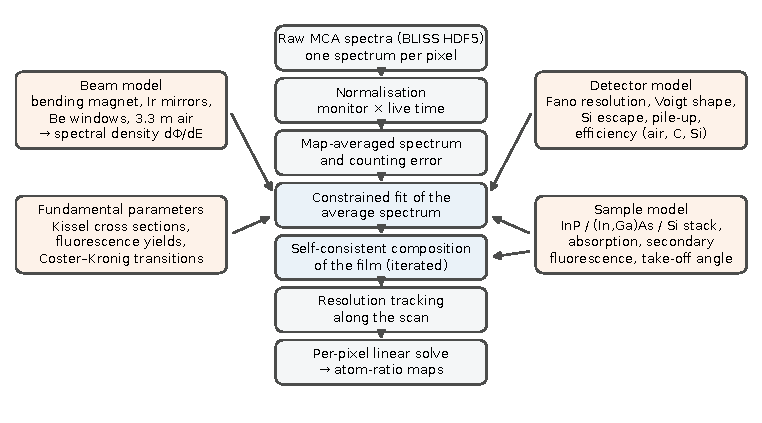
\includegraphics[width=0.92\linewidth]{figures/fig01_workflow.pdf}
\caption{Processing chain. Side boxes are the physical models and data bases; the central column is
the data flow. The two shaded steps are non-linear and run on the map-averaged spectrum; all
per-pixel work is linear.}
\label{fig:workflow}
\end{figure}

The aim is clarity rather than brevity. Figure~\ref{fig:workflow} gives the overview; readers interested only in using the code can skip to
Section~\ref{sec:results} and the recommendations in
Section~\ref{sec:recommendations}.

%=====================================================================================
\section{Experimental setup and data set}\label{sec:setup}
%=====================================================================================
\subsection{Beamline and geometry}
The source is the \qty{0.86}{T} bending magnet of ESRF-EBS (\qty{6.04}{GeV}). Four Ir-coated mirrors at
grazing angles of \numlist{3.062;2.551;3.000;3.000}~\unit{mrad}, two \qty{500}{\micro\metre} Be
windows, and \qty{3.3}{m} of air between the last window and the sample (measured) define the
spectrum at the sample (Section~\ref{sec:beam}). The sample is inclined so that both the incident beam
and the detector axis make an angle of about $40^\circ$ with its surface; these two angles are
\emph{assumed} in this note, not measured, and Section~\ref{sec:uncertainty} shows what that costs.

\subsection{Detector}
The fluorescence detector is a KETEK VITUS H7 silicon-drift detector (SDD) with a \qty{450}{\micro\metre}
Si sensor and a \qty{1}{\micro\metre} carbon (graphene) entrance window, read out by a XIA processor.
Its window is about \qty{20}{cm} from the sample, in air. The MCA has 2048 channels with the linear
calibration
\begin{equation}
E\,[\mathrm{eV}] = \rCalGain\, c - \num{31.263},
\label{eq:calibration}
\end{equation}
so that it covers \qtyrange{0}{20.5}{keV}. The processor records, per pixel, the live time
(\code{xia\_det0\_live\_time}), the real time (\code{xia\_det0\_elapsed\_time}), the trigger (input) and
event (output) count rates and the fractional dead time.

\subsection{Sample}
The sample is a \qty{1.9}{\micro\metre} (In,Ga)As film grown on Si and capped with \qty{50}{nm} of
InP. The densities used are \qty{4.81}{g.cm^{-3}} (InP), \qty{5.5}{g.cm^{-3}} ((In,Ga)As, close to
the mean of GaAs and InAs) and \qty{2.33}{g.cm^{-3}} (Si). The film composition is the unknown; the
cap and the substrate are taken as known.

\subsection{Data set}
The map \code{InPoSi\_v2\_center.h5} is an \rNSlow$\times$\rNFast{} mesh (fast axis \code{xech}, slow
axis \code{yech}, \qty{\rStepUm}{\micro\metre} steps) acquired in \qty{\rCountTime}{s} per point
over \qty{\rScanHours}{h}. On average a pixel records \rCountsPerPixel{} counts, \rTotalCounts{} in
total. The input count rate is \qtyrange{\rIcrMin}{\rIcrMax}{kcps} (mean \qty{\rIcrMean}{kcps}),
the dead-time fraction \rDeadMin--\rDeadMax{} (median \rDeadMed) and the live time
\qtyrange{\rLiveMin}{\rLiveMax}{s} for a real time of \qty{\rRealTime}{s}.

Figure~\ref{fig:data} shows the map-averaged spectrum and the per-pixel normalisation counters.
The spectrum is dominated by Ga K and As K. The In L lines appear between \num{3.1} and
\qty{4.2}{keV} on top of Ar K from air, with Ca K at \qty{3.69}{keV}. A peak at \qty{7.5}{keV}
is mostly the Si escape peak of Ga~K$\alpha$ (Section~\ref{sec:escape}), and Cu K appears at
\qty{8.05}{keV}. Above \qty{12.6}{keV} there are sum peaks (Section~\ref{sec:pileup}) on
a scattered background. The monitor (panel b) decays smoothly with the ring current and jumps
by about \qty{18}{\percent} at three storage-ring refills, about one hour apart, part-way through
rows \rRefillARow, \rRefillBRow{} and \rRefillCRow{} (panel~e).

\begin{figure}[t]
\centering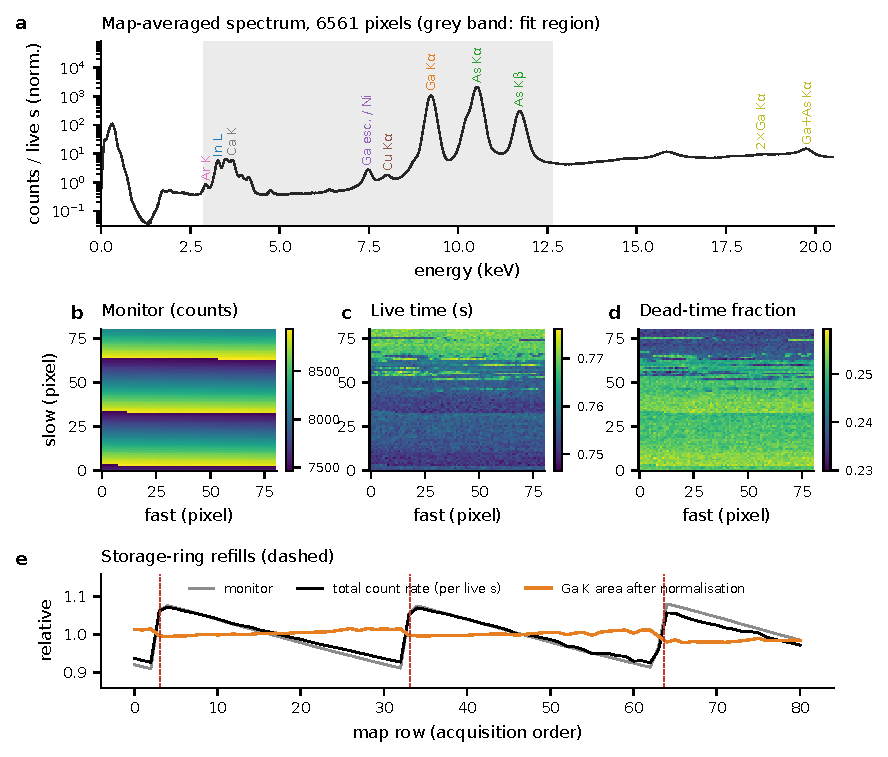
\includegraphics[width=\linewidth]{figures/fig02_data.pdf}
\caption{Data set. (a) Map-averaged, normalised spectrum (logarithmic scale); the grey band is the
analysis region \qtyrange{2.9}{12.6}{keV}. (b--d) Monitor, live time and dead-time fraction per pixel.
(e) Row averages, in acquisition order, of the monitor, of the total count rate per live second, and
of the Ga~K area after normalisation by monitor and live time (Section~\ref{sec:norm}); dashed lines mark
the refills.}
\label{fig:data}
\end{figure}

%=====================================================================================
\section{Overview of the processing chain}\label{sec:overview}
%=====================================================================================
Figure~\ref{fig:workflow} summarises the chain. Three physical models -- the incident beam, the
detector, and the sample -- are combined with tabulated fundamental parameters to predict, for each
element and shell, which lines are emitted, with which relative intensities, and how strongly per unit
concentration. These predictions constrain the fit of the \emph{map-averaged} spectrum. That fit is
non-linear because it adjusts the detector resolution, and it is done once, on very high statistics.
The fitted areas give the composition of the film self-consistently: the matrix correction depends on
the composition, which is iterated. The line shapes are then frozen and every pixel is solved
\emph{linearly} for its line-group areas, which become atom-ratio maps through the converged
sensitivities. One extra step checks whether the detector resolution stayed constant during the scan
and accounts for it if not.


\paragraph{Notation.} $E$ is the incident photon energy and $E_l$ the energy of fluorescence line $l$;
$c$ indexes MCA channels and $i$ pixels; $N_{ic}$ are raw counts; $\mu_k(E)$ is the total mass
attenuation coefficient of layer $k$ (\unit{cm^2.g^{-1}}); $Q_{l}(E)$ the partial (line) fluorescence
cross-section of the emitting element (\unit{cm^2.g^{-1}}); $\varepsilon(E_l)$ the detection
efficiency; $W$ an atomic weight; $w$ a mass fraction and $n$ a number of atoms.

%=====================================================================================
\section{Normalisation and counting statistics}\label{sec:norm}
%=====================================================================================
\subsection{Per-pixel normalisation}
The recorded counts of pixel $i$ are converted into a rate per unit incident flux by dividing by the
monitor (relative to its map mean) and by the live time:
\begin{equation}
y_{ic} = \frac{N_{ic}}{s_i},\qquad s_i = \frac{m_i}{\bar m}\;t^{\mathrm{live}}_i .
\label{eq:norm}
\end{equation}
Dividing by the live time corrects the dead-time losses, whatever their origin, because the XIA live
time is the time during which the processor was able to accept a pulse. The correction is
multiplicative and identical for all channels of a pixel. It therefore cancels exactly in any ratio of
two areas from the same pixel, and so in atom-ratio maps. We checked this numerically: the Ga/As area
ratio map obtained with and without Eq.~\eqref{eq:norm} differs by at most \rInvariance{} (relative).
The normalisation matters for the absolute areas and for the average spectrum, in which pixels are
combined.

\subsection{Uncertainty of the average spectrum}
The map-averaged spectrum is $\bar y_c = N^{-1}\sum_i y_{ic}$. Its \emph{counting} uncertainty follows
from Poisson statistics on the raw counts, $\mathrm{Var}(N_{ic})=N_{ic}$:
\begin{equation}
\sigma_c = \frac{1}{N}\Bigl(\sum_i \frac{N_{ic}}{s_i^2}\Bigr)^{1/2}.
\label{eq:counting}
\end{equation}
This is the weight used to fit $\bar y$. The standard error of the mean across pixels is a different
quantity: it also contains real pixel-to-pixel variation, which is signal as far as the average is
concerned. Here, at the peak, the two happen to be almost equal (\rCntErrPeak{} and \rSemPeak{} of the peak height) because the map is close to homogeneous; on a heterogeneous map they can differ by an
order of magnitude.

\subsection{Monitor behaviour at storage-ring refills}\label{sec:refills}
Figure~\ref{fig:data}e tests the monitor. Before normalisation, the row-averaged count rate follows the
monitor closely (correlation \rRateMonCorr). Its row-to-row spread drops from \qty{\rRateRowSpread}{\percent}
to \qty{\rRateMonRowSpread}{\percent} after division by the monitor. The correction is not perfect at
the refills, however: the monitor jumps by \qty{\rRefillAMon}{\percent}, \qty{\rRefillBMon}{\percent} and
\qty{\rRefillCMon}{\percent}, while the fluorescence count rate jumps by only
\qty{\rRefillARate}{\percent}, \qty{\rRefillBRate}{\percent} and \qty{\rRefillCRate}{\percent}.
The normalised Ga~K area therefore steps by \qty{\rRefillAGa}{\percent}, \qty{\rRefillBGa}{\percent} and
\qty{\rRefillCGa}{\percent} (comparing the 200 pixels on either side), which is visible as
horizontal bands in the area maps (Fig.~\ref{fig:maps}a,b). The Ga/As ratio steps by only
\qty{\rRefillARatio}{\percent}, \qty{\rRefillBRatio}{\percent} and \qty{\rRefillCRatio}{\percent}.
The monitor over-responds: \qtyrange{\rMonOverMin}{\rMonOverMax}{\percent} of its jump is not seen by the fluorescence. A dark
offset or a non-linearity of the monitor, or a change of the focused beam after a refill (heat load on
the optics), would each produce this; the present data cannot distinguish them. Absolute
areas therefore carry a systematic error of about \qty{2}{\percent} correlated with the refill cycle,
whereas ratios are immune.

%=====================================================================================
\section{Incident white-beam spectrum}\label{sec:beam}
%=====================================================================================
\subsection{Source}
The flux of a bending magnet, integrated over the vertical opening angle, per horizontal angle and per
\qty{0.1}{\percent} bandwidth, is \citep{Schwinger1949,Kim1989,XDB2009}
\begin{equation}
\frac{\dd\dot N}{\dd\theta}\Big|_{0.1\%\,\mathrm{BW}} = 2.457\times10^{13}\,E_e[\mathrm{GeV}]\,I[\mathrm{A}]\;G_1(y),
\qquad G_1(y) = y\int_y^\infty K_{5/3}(x)\,\dd x,\qquad y = \frac{E}{E_c},
\label{eq:schwinger}
\end{equation}
with the critical energy $E_c[\mathrm{keV}] = 0.665\,E_e^2[\mathrm{GeV}]\,B[\mathrm{T}] = \qty{\rEc}{keV}$.
Only the spectral shape $G_1(y)$ enters any result of this note, since every quantity used is a
ratio.\footnote{The implementation (\code{BendingMagnetSource.spectral\_flux}) uses the prefactor
$1.327\times10^{13}E_e^2 I$, which is the on-axis constant of the angular density; it differs from
Eq.~\eqref{eq:schwinger} by a constant factor and is irrelevant for ratios, but must be corrected
before quoting absolute fluxes.} The vertically integrated form is appropriate because the beamline
accepts the full vertical opening angle.

\subsection{Optics and absorbers}
Each mirror is described by its Fresnel reflectivity for $s$ polarisation (the mirrors deflect vertically
and the radiation is horizontally polarised) \citep{Parratt1954,AlsNielsen2011}:
\begin{equation}
R(E,\theta) = \left|\frac{\sin\theta - q}{\sin\theta + q}\right|^2,\qquad q=\sqrt{n^2-\cos^2\theta},\qquad
n = 1-\delta(E)+\mathrm{i}\beta(E),
\label{eq:fresnel}
\end{equation}
with the refractive index of Ir (\qty{22.56}{g.cm^{-3}}) from xraylib \citep{Brunetti2004,Schoonjans2011}.
Interface roughness $\sigma$ would multiply the reflection amplitude by the Névot--Croce factor
$\exp(-2k_{z0}k_{z1}\sigma^2)$ \citep{Nevot1980}, i.e.\ $R$ by $\exp[-4k_0^2\sin\theta\,\mathrm{Re}(q)\,\sigma^2]$.
The roughness is unknown and set to zero here.
Windows and air transmit $T=\exp[-(\mu/\rho)\rho t]$, with total attenuation coefficients and,
for air, the density of an ideal gas of N, O, Ar and C at \qty{20}{\degreeCelsius} and
\qty{1013.25}{hPa}. The spectrum at the sample is
\begin{equation}
\Phi(E) = \frac{\dd\dot N}{\dd\theta}(E)\;\prod_{j} T_j(E),
\label{eq:phi}
\end{equation}
shown in Fig.~\ref{fig:beam}a,b. The mirrors cut off above about \qty{28}{keV}; the \qty{3.3}{m}
of air, not the Be windows, sets the low-energy end. The Ir L edges imprint three small steps
between \num{11.2} and \qty{13.4}{keV}. The band where $\Phi$ exceeds \qty{10}{\percent} of its maximum is
\qtyrange{\rBandTenLo}{\rBandTenHi}{keV} (\qtyrange{\rBandOneLo}{\rBandOneHi}{keV} at \qty{1}{\percent}).

\subsection{From flux per bandwidth to spectral density}\label{sec:jacobian}
Eq.~\eqref{eq:schwinger} is a flux per \qty{0.1}{\percent} bandwidth, i.e.\ per interval
$\dd E = 10^{-3}E$. Any integral over photon energy needs the spectral density per unit energy,
\begin{equation}
\frac{\dd\Phi}{\dd E} = \frac{\Phi_{0.1\%}(E)}{10^{-3}\,E},
\label{eq:jacobian}
\end{equation}
which peaks at \qty{\rPeakKeV}{keV} instead of \qty{\rPeakBW}{keV} (Fig.~\ref{fig:beam}c). Forgetting this
Jacobian over-weights high energies by a factor $E$. For the bare Ga/As sensitivity ratio
$k=\int Q_{\mathrm{As}}\,\dd\Phi\, W_\mathrm{As} / \int Q_{\mathrm{Ga}}\,\dd\Phi\, W_\mathrm{Ga}$ (K lines,
no detector or matrix) it gives \rkBW{} instead of \rkKeV, a bias of \qty{\rkJacobianBias}{\percent} on the
Ga/As ratio.

\begin{figure}[t]
\centering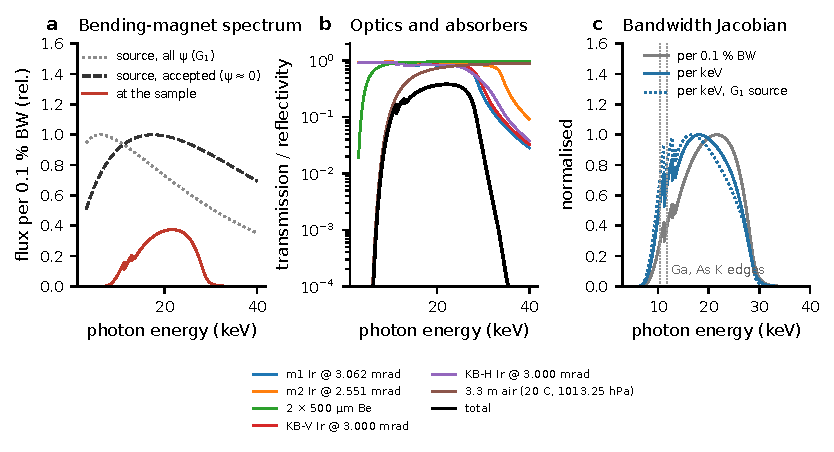
\includegraphics[width=\linewidth]{figures/fig03_beam.pdf}
\caption{Incident spectrum. (a) Bending-magnet flux per \qty{0.1}{\percent} bandwidth at the source
and after the optics, normalised to the source maximum. (b) Transmission or reflectivity of each
element and their product. (c) The same spectrum per \qty{0.1}{\percent} bandwidth and per unit energy
(Eq.~\ref{eq:jacobian}), each normalised to its maximum; the dotted lines mark the Ga and As K edges.}
\label{fig:beam}
\end{figure}

%=====================================================================================
\section{Detector response}\label{sec:detector}
%=====================================================================================
\subsection{Energy calibration}
The linear calibration of Eq.~\eqref{eq:calibration} is taken from the beamline and held fixed in the
fit. Its stability is checked by the centroid analysis of Section~\ref{sec:resolution}: the Ga~K$\alpha$
centroid moves by \qty{\rCentroidRange}{eV} at most over the scan and shows no step. Its absolute accuracy
has not been tested beyond the quality of the fit; refining gain and offset is one of the
recommendations of Section~\ref{sec:recommendations}.

\subsection{Resolution and line shape}
The Gaussian width of a line combines an electronic-noise term and the Fano-limited fluctuation of the
number of electron--hole pairs \citep{Fano1947,Knoll2010}:
\begin{equation}
\sigma^2(E) = \sigma_\mathrm{n}^2 + F\,w\,E,\qquad \mathrm{FWHM} = 2.3548\,\sigma,
\label{eq:resolution}
\end{equation}
with $w$ the mean pair-creation energy. Each line is a Voigt profile, the convolution of this Gaussian
with a Lorentzian of half-width $\gamma$ that stands for the natural line width. $\sigma_\mathrm{n}$,
$F$ and $\gamma$ are common to all lines and fitted on the average spectrum.
The implementation uses $w=\qty{3.85}{eV}$; the measured value for Si at room temperature is
$w=\qty{3.66\pm0.03}{eV}$ \citep{Scholze1998}. Only the product $Fw$ is determined by the data, so the
choice only rescales the reported Fano factor (\rFano{} with \qty{3.85}{eV} corresponds to \rFanoW{}
with \qty{3.66}{eV}).
The fit gives $\sigma_\mathrm{n}=\qty{\rNoise}{eV}$, $F=\rFano$ and $\gamma=\qty{\rGamma}{eV}$, i.e.\
\qty{\rFwhmMn}{eV} FWHM at Mn~K$\alpha$ and \qty{\rFwhmGa}{eV} at Ga~K$\alpha$. That is broader than
the \qty{129}{eV} quoted at optimum shaping, as expected at \qty{100}{kcps}, where a short peaking
time is used. Over \qtyrange{3}{12}{keV} the noise and Fano terms are strongly correlated, and their
values should be read as an effective resolution law, not as detector physics. The Lorentzian width is
larger than natural widths of K lines (a few eV). It partly absorbs a low-energy tail that the model
does not contain (Section~\ref{sec:fit}).

\subsection{Detection efficiency}
The probability that a photon emitted towards the detector is recorded in the full-energy peak or its
escape peak is
\begin{equation}
\varepsilon(E_l) = \e^{-\mu_\mathrm{air}(E_l)\rho_\mathrm{air}d_\mathrm{air}}\;
\e^{-\mu_\mathrm{C}(E_l)\rho_\mathrm{C}d_\mathrm{C}}\;
\bigl[1-\e^{-\tau_\mathrm{Si}(E_l)\rho_\mathrm{Si}d_\mathrm{Si}}\bigr],
\label{eq:efficiency}
\end{equation}
using total attenuation coefficients along the path (any interaction removes the photon) and the
photoelectric coefficient $\tau$ in the sensor (a scattered photon does not deposit its full energy).
No dead layer is assumed. Figure~\ref{fig:detector}a shows the factors for $d_\mathrm{air}=\qty{20}{cm}$,
$d_\mathrm{C}=\qty{1}{\micro\metre}$ and $d_\mathrm{Si}=\qty{450}{\micro\metre}$. The efficiency is
\rEffGa{} at Ga~K$\alpha_1$, \rEffAs{} at As~K$\alpha_1$, \rEffAsKb{} at As~K$\beta_1$, but only
\rEffIn{} at In~L$\alpha_1$. The air path dominates that number: one more centimetre of air
multiplies the In~L$\alpha_1$ efficiency by \rEffInPerCm{} and the Ga~K$\alpha_1$ efficiency by
\rEffGaPerCm{} (Fig.~\ref{fig:detector}b). The local pressure matters too: \qty{990}{hPa} instead
of \qty{1013}{hPa} raises the In~L$\alpha_1$ efficiency by a factor \rEffInLowP.
This single factor is the main uncertainty of any quantification based on soft lines
(Section~\ref{sec:uncertainty}).

\begin{figure}[t]
\centering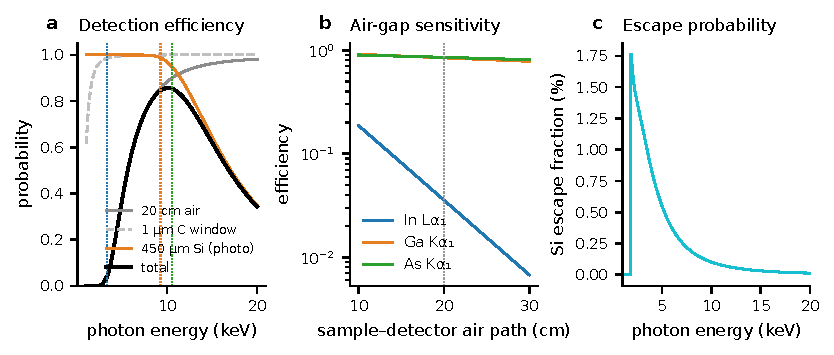
\includegraphics[width=\linewidth]{figures/fig04_detector.pdf}
\caption{Detector. (a) Transmission of \qty{20}{cm} of air and of the \qty{1}{\micro\metre} carbon
window, photo-absorption in \qty{450}{\micro\metre} Si, and the resulting efficiency
(Eq.~\ref{eq:efficiency}); dotted lines mark In~L$\alpha_1$, Ga~K$\alpha_1$ and As~K$\alpha_1$.
(b) Efficiency versus sample--detector air path. (c) Total Si~K escape fraction (Eq.~\ref{eq:escape}).}
\label{fig:detector}
\end{figure}

\subsection{Silicon escape peaks}\label{sec:escape}
A photon absorbed in the Si K shell near the entrance of the sensor may be followed by a Si~K X-ray
that leaves the crystal; the event is then recorded at $E-E_X$. For normal incidence on a thick sensor
the escape fraction is \citep{ReedWare1972}
\begin{equation}
f_X(E) = \tfrac12\,\omega_K\,\frac{\tau_K(E)}{\tau(E)}\,p_X
\Bigl[1-\frac{\mu(E_X)}{\tau(E)}\ln\Bigl(1+\frac{\tau(E)}{\mu(E_X)}\Bigr)\Bigr],
\label{eq:escape}
\end{equation}
with $\omega_K$ the Si K fluorescence yield, $\tau_K/\tau$ the K-shell share of photo-absorption at $E$,
$p_X$ the fraction of K$\alpha$ or K$\beta$ among Si K emissions, $\tau(E)$ the photo-absorption
coefficient of Si at $E$ and $\mu(E_X)$ the attenuation of the escaping line. The fraction reaches
\qty{\rEscMax}{\percent} just above the Si K edge and falls to \qty{\rEscIn}{\percent} at In~L$\alpha$ and
\qty{\rEscGa}{\percent} at Ga~K$\alpha$ (Fig.~\ref{fig:detector}c). Every line of the model carries
its escape companions with this fraction and the resolution of the deposited energy $E-E_X$, with no
extra free parameter. The group area then counts every photon absorbed in the sensor, consistently with
Eq.~\eqref{eq:efficiency}.

The Ga~K$\alpha$ escape peak lies at \qty{7.51}{keV}, \qty{30}{eV} from Ni~K$\alpha$ (\qty{7.48}{keV}).
Without escape peaks the fit attributes \qty{\rNiNoEsc}{\counts\per\second} to Ni~K. With them, the Ni
area drops to \qty{\rNiEsc}{\counts\per\second} (Fig.~\ref{fig:escape}a). The remainder is either
genuine Ni or an underestimate of the escape fraction. Eq.~\eqref{eq:escape} ignores escape through the
sides of a collimated sensor and the incomplete charge collection near its entrance window.
The overall $\chi^2$ does not improve with the escape peaks (\rChiNoEsc{} without, \rChiEsc{} with):
the misfit around \qty{8.8}{keV}, where the As~K$\alpha$ escape adds to the unmodelled low-energy
tail of Ga~K$\alpha$, outweighs the gain at \qty{7.5}{keV}. The escape term is kept on physical
grounds.

\begin{figure}[t]
\centering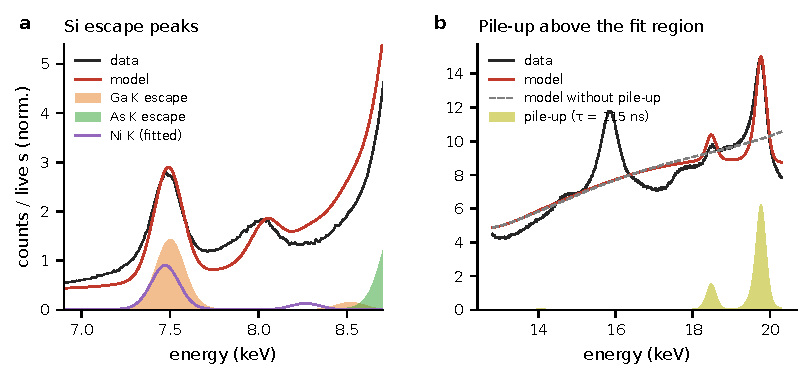
\includegraphics[width=\linewidth]{figures/fig07_escape_pileup.pdf}
\caption{(a) Region of the Si escape peaks of Ga~K and As~K. The escape components (shaded) are tied
to their parent lines; the purple line is the Ni~K group still fitted. (b) Extended fit up to
\qty{20.3}{keV} with and without the pile-up term (Eq.~\ref{eq:pileup}); the shaded areas are the
predicted 2$\times$Ga~K$\alpha$ and Ga~K$\alpha$+As~K$\alpha$ sum peaks for the fitted resolving time.}
\label{fig:escape}
\end{figure}

\subsection{Pulse pile-up}\label{sec:pileup}
Two photons arriving within the pulse-pair resolving time $\tau_\mathrm{pp}$ of the pile-up inspector
are recorded as one event at the sum of their energies. For Poisson arrivals, and to first order, the
pile-up spectrum of a pixel is \citep{Statham1977}
\begin{equation}
N^\mathrm{pp}_{i}(E) = \frac{\tau_\mathrm{pp}}{t_i^\mathrm{real}}\,(x_i\otimes x_i)(E),\qquad
(x\otimes x)(E) = \sum_{E_1+E_2=E} x(E_1)\,x(E_2),
\label{eq:pileup}
\end{equation}
where $x_i$ is the measured spectrum of the pixel and the sum runs over ordered pairs. The
self-convolution is computed per pixel by FFT over the full MCA range, with the calibration
offset counted twice and the diagonal term made unbiased ($x_c(x_c-1)$). Pile-up goes as the square of
the local rate, so the template for the average spectrum is the average of the per-pixel
$N^\mathrm{pp}_i/s_i$, not the self-convolution of the average. Pile-up removes the two parent events
regardless of their energies, so it does not bias line ratios; its effect is the sum peaks, which other
components of the model would otherwise absorb.

The main sum peaks (\num{18.5} and \qty{19.8}{keV}) lie above the analysis region, so
$\tau_\mathrm{pp}$ is fitted once over \qtyrange{2.9}{20.3}{keV} (background order 5) and then held
fixed. This gives $\tau_\mathrm{pp} = \qty{\rTau\pm\rTauErr}{\micro\second}$ (statistical) and lowers
$\chi^2_\nu$ of that extended fit from \rTauChiWithout{} to \rTauChiWith{} (Fig.~\ref{fig:escape}b).
At the mean input rate the probability that a given event is piled up is about
\qty{\rPairProb}{\percent}. A single $\tau_\mathrm{pp}$ describes the Ga+As sum peak well but
overestimates the 2$\times$Ga~K$\alpha$ peak, consistent with a resolving time that depends on the
energies of the two pulses \citep{Statham1977}. A broad peak at \qty{15.8}{keV}, with weaker features
near \num{14.5} and \qty{17.5}{keV}, is not part of the model. Its energy matches Zr~K$\alpha$
(\qty{15.78}{keV}, with K$\beta$ at \qty{17.67}{keV}), but a Bragg reflection of the white beam by the
single-crystal sample reaching the detector cannot be excluded. It lies outside the analysis region.

%=====================================================================================
\section{Fundamental parameters and line groups}\label{sec:fp}
%=====================================================================================
\subsection{Line fluorescence cross-sections}
For each element and each shell family (K, L) the model contains every transition listed by xraylib
under its IUPAC name (e.g.\ \code{KL3}, \code{L3M5}). Siegbahn aliases and composite macros
(\code{KA}, \code{LA}) are excluded so that no intensity is counted twice. The emission of line $l$
of element $i$ per unit mass, for an incident photon of energy $E$, is the partial fluorescence
cross-section
\begin{equation}
Q_{il}(E) = \Bigl[\tau_{L_3}(E) + f_{23}\tau_{L_2}(E) + (f_{13}+f_{12}f_{23})\tau_{L_1}(E)\Bigr]\,
\omega_{L_3}\,p_{l}\qquad(\text{for an }L_3\text{ line}),
\label{eq:Q}
\end{equation}
with subshell photo-ionisation cross-sections $\tau$ (Kissel), Coster--Kronig transfer probabilities $f$,
fluorescence yields $\omega$ and radiative branching ratios $p_l$
(\code{CS\_FluorLine\_Kissel} \citep{Brunetti2004,Schoonjans2011,Krause1979,Campbell2003,Elam2002}).
K lines have the same form without the transfer terms. $Q$ is comparable across subshells, which
radiative rates alone are not. That matters for L lines, which originate from three subshells with
different edges.

\subsection{Flux-weighted line strengths}
Under white-beam excitation the strength of line $l$, before matrix effects, is
\begin{equation}
s_{il} = \varepsilon(E_l)\int Q_{il}(E)\,\frac{\dd\Phi}{\dd E}\,\dd E ,
\label{eq:strength}
\end{equation}
integrated with the trapezoidal rule on a \qty{10}{eV} grid from \num{3} to \qty{40}{keV}. The trapezoidal
rule cannot overshoot at the edge discontinuity. The lines of a group (element, family) whose strength
exceeds \qty{0.5}{\percent} of the strongest are kept, and each gets a fixed relative intensity
$r_l = s_{il}/s_{i,\mathrm{ref}}$. For the stack of Section~\ref{sec:matrix}, $s$ is replaced by the
sensitivity of Eq.~\eqref{eq:emission}.

Table~\ref{tab:levels} shows how the successive physics levels change the predicted line pattern. An
effective excitation energy of \qty{20}{keV} gives In~L$\beta_1$/L$\alpha_1$ = \rInLbScalar. Weighting
by the white beam changes the share of the three L subshells, and the detector efficiency, which is
much higher at L$\beta_1$ (\qty{3.49}{keV}) than at L$\alpha_1$ (\qty{3.29}{keV}), nearly doubles the
ratio. Self-absorption in the film raises it further, because the film absorbs L$\alpha_1$ more strongly
than L$\beta_1$.

\begin{table}[t]
\centering
\caption{Predicted relative intensities (to the reference line of the group) and reduced $\chi^2$ of the
average-spectrum fit at increasing levels of physics. All fits include escape and pile-up.}
\label{tab:levels}
\begin{tabular}{lcccccc}
\toprule
level & \multicolumn{3}{c}{In L, relative to L$_3$M$_5$ (L$\alpha_1$)} & \multicolumn{2}{c}{As K, relative to KL$_3$} & $\chi^2_\nu$\\
\cmidrule(lr){2-4}\cmidrule(lr){5-6}
 & L$_2$M$_4$ (L$\beta_1$) & L$_3$N$_5$ (L$\beta_2$) & L$_1$M$_3$ (L$\beta_3$) & KL$_2$ & KM$_3$ & \\
\midrule
$E_\mathrm{eff}=\qty{20}{keV}$ & \rInLbScalar & \rInLbiiiScalar & \rInLbivScalar & \rAsKaiiScalar & \rAsKbScalar & \rChiScalar\\
white beam & \rInLbWhite & \rInLbiiiWhite & \rInLbivWhite & \rAsKaiiWhite & \rAsKbWhite & \rChiWhite\\
+ detector efficiency & \rInLbWhiteEff & \rInLbiiiWhiteEff & \rInLbivWhiteEff & \rAsKaiiWhiteEff & \rAsKbWhiteEff & \rChiWhiteEff\\
+ sample (stack) & \rInLbMatrix & \rInLbiiiMatrix & \rInLbivMatrix & \rAsKaiiMatrix & \rAsKbMatrix & \rChiMatrix\\
\bottomrule
\end{tabular}
\end{table}

%=====================================================================================
\section{Sample model: absorption and secondary fluorescence in a layer stack}\label{sec:matrix}
%=====================================================================================
\subsection{Primary fluorescence}
Layers are numbered from the surface, $k=0,1,\dots$; layer $k$ has mass thickness $M_k=\rho_k t_k$
(infinite for a bulk last layer). With incidence and take-off angles $\psi_\mathrm{in}$ and
$\psi_\mathrm{out}$ measured from the surface, define
\begin{equation}
a_k(E)=\frac{\mu_k(E)}{\sin\psi_\mathrm{in}},\quad b_k=\frac{\mu_k(E_l)}{\sin\psi_\mathrm{out}},\quad
F(c;M)=\frac{1-\e^{-cM}}{c},\quad G(x,y;M)=\frac{\e^{-yM}-\e^{-xM}}{x-y}.
\end{equation}
The primary sensitivity of line $l$ of element $i$ in layer $k$, per unit mass fraction, is
\citep{Sherman1955,Shiraiwa1966,deBoer1990}
\begin{equation}
P^k_{il} = T^k_\mathrm{out}\int \frac{\dd\Phi}{\dd E}\,\frac{Q_{il}(E)}{\sin\psi_\mathrm{in}}\,
T^k_\mathrm{in}(E)\,F\bigl(a_k(E)+b_k;M_k\bigr)\,\dd E ,
\label{eq:primary}
\end{equation}
with the overlayer transmissions $T^k_\mathrm{in}=\exp(-\sum_{c<k}a_cM_c)$ and
$T^k_\mathrm{out}=\exp(-\sum_{c<k}b_cM_c)$. The ratio of $P^k$ to its value without any absorption
($F\to M_k$, no overlayers) is the absorption factor $A$.

\subsection{Secondary fluorescence}
Line $j$ of element $e$, excited by the beam in layer $\alpha$, is emitted isotropically and can be
absorbed by element $i$ in layer $k$, which then emits line $l$. Writing $u=\cos\vartheta$ for the
direction of the secondary photon and $\kappa_c = \mu_c(E_j)/u$, the depth integrals are closed-form
for every $u$, and \citep{Shiraiwa1966,Mantler1986,deBoer1990}
\begin{equation}
S^k_{il} = T^k_\mathrm{out}\sum_{\alpha,\,e,\,j}\tfrac12\,Q_{il}(E_j)\,w^\alpha_e
\int\frac{\dd\Phi}{\dd E}\,\frac{Q_{ej}(E)}{\sin\psi_\mathrm{in}}\,T^\alpha_\mathrm{in}(E)
\int_0^1 K_{\alpha k}(E,u)\,\frac{\dd u}{u}\,\dd E ,
\label{eq:secondary}
\end{equation}
with the kernels
\begin{align}
K_{kk} &= \frac{F(a_k+\kappa_k)-F(a_k+b_k)}{b_k-\kappa_k} + \frac{F(b_k+\kappa_k)-F(a_k+b_k)}{a_k-\kappa_k}
&&\text{(same layer)},\nonumber\\
K_{\alpha k} &= G(a_\alpha,\kappa_\alpha;M_\alpha)\;\e^{-\sum_{\alpha<c<k}\kappa_cM_c}\;F(b_k+\kappa_k;M_k)
&&(\alpha<k,\ \text{downward}),\label{eq:kernels}\\
K_{\alpha k} &= F(a_\alpha+\kappa_\alpha;M_\alpha)\;\e^{-\sum_{k<c<\alpha}\kappa_cM_c}\;G(b_k,\kappa_k;M_k)
&&(\alpha>k,\ \text{upward}).\nonumber
\end{align}
The same-layer kernel is the closed form of
$\int_0^M\!\int_0^M \e^{-am-bm'-\kappa|m-m'|}\dd m\,\dd m'$; its removable singularities at $b=\kappa$
and $a=\kappa$ are handled by the derivative of $F$. The $u$ integral is done on a logarithmic grid
of 160 points, which resolves the grazing paths that dominate in thin films. The energy integral
uses a coarser \qty{40}{eV} grid. For a single bulk layer Eq.~\eqref{eq:secondary} reduces to the
classical Shiraiwa--Fujino expression. Tertiary fluorescence, excitation by scattered radiation and
interface roughness are not included.

The implementation was checked against brute-force numerical integration of the double depth integral
(agreement to \num{1e-6}), against the classical bulk expression (\num{4e-4}) and against an independent
estimate of the Ga~K enhancement in a \qty{200}{nm} film (\qty{1.20}{\percent} against \qty{1.19}{\percent}).
Splitting a layer into two identical sublayers changes nothing to within $10^{-10}$.

\subsection{Recorded intensity}
The intensity of line $l$ recorded from the whole stack is
\begin{equation}
I_{il} \propto \varepsilon(E_l)\sum_k w^k_i\,\bigl(P^k_{il}+S^k_{il}\bigr).
\label{eq:emission}
\end{equation}
Figure~\ref{fig:matrix} shows how absorption and secondary fluorescence evolve with the thickness of an
In$_{0.5}$Ga$_{0.5}$As layer alone. At \qty{1.9}{\micro\metre} the absorption factor is
\rCurveAbsGaNineteen{} for Ga~K$\alpha$ but \rCurveAbsInNineteen{} for In~L$\alpha$, and the secondary
fluorescence adds \qty{\rCurveSFGaNineteen}{\percent} to Ga~K$\alpha$ (excited by As~K) and
\qty{\rCurveSFInNineteen}{\percent} to In~L$\alpha$ (excited by As~K and Ga~K). As~K is not enhanced.
Both effects grow without saturation up to \qty{10}{\micro\metre} (Ga
\qty{\rCurveSFGaTen}{\percent}, In \qty{\rCurveSFInTen}{\percent}): the film is not thin for any of the
lines of interest.

\begin{figure}[t]
\centering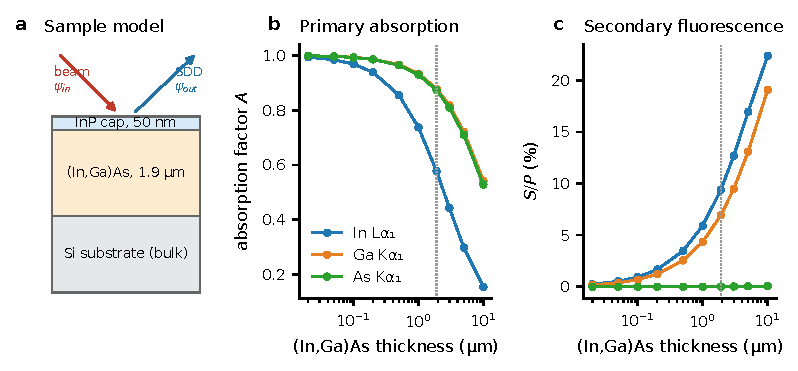
\includegraphics[width=\linewidth]{figures/fig05_matrix.pdf}
\caption{Sample model. (a) Stack and geometry. (b) Absorption factor (primary intensity relative to a
non-absorbing layer) and (c) secondary-to-primary ratio of In~L$\alpha_1$, Ga~K$\alpha_1$ and
As~K$\alpha_1$ for an In$_{0.5}$Ga$_{0.5}$As layer (\qty{5.5}{g.cm^{-3}}) of varying thickness,
$\psi_\mathrm{in}=\psi_\mathrm{out}=40^\circ$; the dotted line marks \qty{1.9}{\micro\metre}.}
\label{fig:matrix}
\end{figure}

%=====================================================================================
\section{Fit of the map-averaged spectrum}\label{sec:fit}
%=====================================================================================
\subsection{Model}
Over the analysis region (channels \rRoiLo--\rRoiHi, \qtyrange{2.9}{12.6}{keV}) the model is
\begin{equation}
\hat y(c) = \sum_{k=0}^{K} \beta_k u^k + \tau_\mathrm{pp}\,\bar N^\mathrm{pp}(c) +
\sum_g A_g\sum_{l\in g} r_l\Bigl[\bigl(1-\textstyle\sum_X f_X\bigr)V(c-c_l;\sigma_l,\gamma)
+\textstyle\sum_X f_X\,V(c-c_{l,X};\sigma_{l,X},\gamma)\Bigr],
\label{eq:model}
\end{equation}
with $u\in[-1,1]$ the scaled channel, a polynomial background of order $K=3$, $V$ a unit-area Voigt
profile in channel units, $c_l$ the channel of line $l$ from Eq.~\eqref{eq:calibration}, $\sigma_l$
from Eq.~\eqref{eq:resolution}, and $A_g$ the area of the reference line of group $g$ (escape
included). The relative intensities $r_l$ and escape fractions $f_X$ are fixed by
Sections~\ref{sec:detector}--\ref{sec:matrix}; the pile-up term $\bar N^\mathrm{pp}$ is the
average template of Eq.~\eqref{eq:pileup} with $\tau_\mathrm{pp}$ fixed. The free parameters are the
background coefficients, one area per group (In~L, Ga~K, As~K, Cu~K, Ni~K, Ca~K, Ar~K), and
$\sigma_\mathrm{n}$, $F$, $\gamma$: \rNFree{} parameters for \rNLines{} lines in \rNGroups{} groups.
The fit is a weighted least-squares problem with the counting errors of Eq.~\eqref{eq:counting}
(trust-region reflective algorithm with bounds, \code{scipy.optimize.curve\_fit}).

\subsection{Result}
Figure~\ref{fig:fit} shows the fit. The r.m.s.\ residual is \qty{\rResidRms}{\percent} of the
maximum, but $\chi^2_\nu = \rChi$ over \rNChan{} channels. With \rTotalCounts{} counts in the
average, the counting errors are tiny and $\chi^2$ is set by systematic line-shape deviations. The
residuals show their structure: excess counts on the low-energy side of each strong peak (incomplete
charge collection, i.e.\ a tail and shelf that a Voigt profile does not have \citep{Phillips1976}) and
the corresponding overshoot of the fitted Lorentzian wings between the peaks. The fitted areas
(\unit{\counts\per\second}, per unit relative monitor) are
In~L \rAreaIn{}$\pm$\rAreaErrIn, Ga~K \rAreaGa{}$\pm$\rAreaErrGa, As~K \rAreaAs{}$\pm$\rAreaErrAs,
Cu~K \rAreaCu, Ni~K \rAreaNi, Ca~K \rAreaCa{} and Ar~K \rAreaAr; the quoted errors are
statistical only. Successive physics levels change $\chi^2_\nu$ only moderately
(Table~\ref{tab:levels}). The white-beam and efficiency levels alone slightly increase it, and the full sample model gives the
lowest value. This suggests that the predicted In~L pattern becomes consistent with the data only
once self-absorption is included.

\begin{figure}[t]
\centering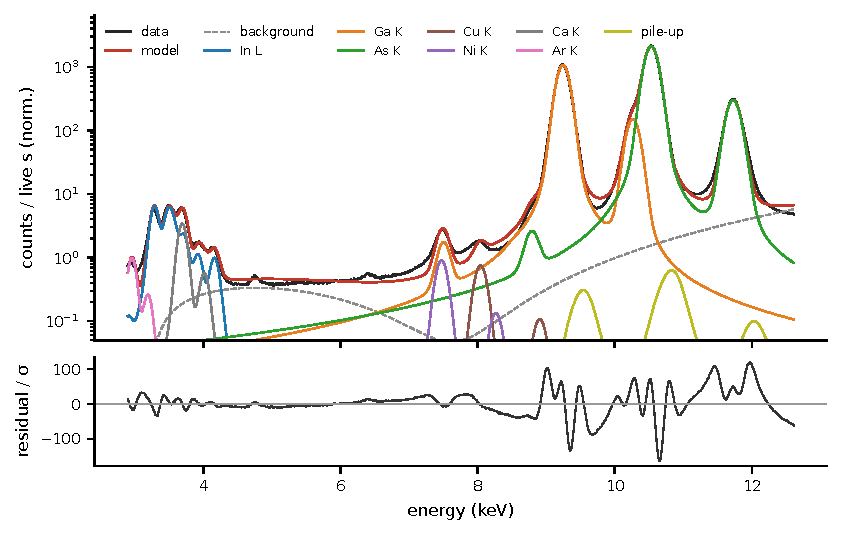
\includegraphics[width=\linewidth]{figures/fig06_fit.pdf}
\caption{Fit of the map-averaged spectrum with the full model (white beam, detector efficiency, stack
with secondary fluorescence, escape, fixed pile-up). Coloured lines are the line groups including their
escape peaks; the lower panel is the residual in units of the counting error.}
\label{fig:fit}
\end{figure}

%=====================================================================================
\section{Self-consistent quantification of a buried layer}\label{sec:quant}
%=====================================================================================
\subsection{Single layer}
For a homogeneous sample, the reference-line area of group $g$ is $A_g\propto w_g s_g$, with
$s_g = \varepsilon(P+S)$ the sensitivity per unit mass fraction. With $w = nW/\sum nW$, the atom ratio of
two elements is
\begin{equation}
\frac{n_a}{n_b} = \frac{A_a}{A_b}\,\frac{s_b\,W_b}{s_a\,W_a}.
\label{eq:numberratio}
\end{equation}
Because $s$ depends on the composition through absorption and secondary fluorescence,
Eq.~\eqref{eq:numberratio} is iterated: start from a nominal composition, compute the ratios, rebuild
the layer, recompute $s$, until the ratios change by less than $10^{-6}$ \citep{Criss1968}.

\subsection{Target layer in a stack}
When other layers emit the same lines (here In~L from the InP cap), the measured intensity is
\begin{equation}
A_g \propto w^t_g s^t_g + C_g,\qquad C_g = \sum_{k\neq t} w^k_g s^k_g ,
\end{equation}
where $t$ is the target layer and the other layers have known composition. Relative to the reference
group $r$ (As~K),
\begin{equation}
w^t_i = \frac{(A_i/A_r)\,(w^t_r s^t_r + C_r) - C_i}{s^t_i},
\label{eq:stackquant}
\end{equation}
and the atom ratios follow from the mass fractions. The absolute mass fraction of the reference enters
once $C\neq0$, so unmeasured elements of the target layer must be fixed or neglected. Density and
thicknesses are held fixed; the iteration converged in \rIter{} steps.

\subsection{Result on the average spectrum}
The film composition per As atom is
\begin{equation}
n_\mathrm{Ga}/n_\mathrm{As} = \rxGa,\qquad n_\mathrm{In}/n_\mathrm{As} = \rxIn,\qquad
(n_\mathrm{Ga}+n_\mathrm{In})/n_\mathrm{As} = \rClosure .
\end{equation}
Table~\ref{tab:quant} lists the matrix terms. The Ga/As ratio is close to the raw area ratio
($k=\rkGa$) because the absorption of Ga~K$\alpha$ and As~K$\alpha$ is similar (\rAbsGa{} and \rAbsAs) and
the \qty{\rSFGa}{\percent} secondary enhancement of Ga by As~K ($\mathrm{KL_3}$ \qty{\rSFGaAsKLiii}{\percent},
$\mathrm{KL_2}$ \qty{\rSFGaAsKLii}{\percent}, $\mathrm{KM_3}$ \qty{\rSFGaAsKMiii}{\percent}) is
compensated by the Ga/As cross-section ratio. Without the sample model (white beam and efficiency
only) the same areas give $n_\mathrm{Ga}/n_\mathrm{As}=\rxGaNoMatrix$, i.e.\ the sample model changes the
result by \qty{\rMatrixEffect}{\percent}.

The InP cap matters only for In: it emits \qty{\rCapInFrac}{\percent} of the modelled In~L intensity and
transmits \rCapTIn{} of In~L$\alpha$ and more than \rCapTGa{} of Ga and As~K$\alpha$. Ignoring the cap
gives $n_\mathrm{In}/n_\mathrm{As} = \rxInNoCap$ (closure \rClosureNoCap) and leaves Ga/As unchanged
(\rxGaNoCap). The closure deficit is therefore not a cap effect: to bring the closure to~1 with the
cap alone, it would have to be about \qty{500}{nm} thick (closure \rCapScanFive{} at \qty{500}{nm},
against \rClosure{} at \qty{50}{nm}).

\begin{table}[t]
\centering
\caption{Matrix terms of the converged quantification for the reference line of each group in the
(In,Ga)As film: absorption factor $A$, secondary-to-primary ratio $S/P$, fraction of the modelled
intensity emitted by the other layers, and transmission of the \qty{50}{nm} InP cap.}
\label{tab:quant}
\begin{tabular}{lcccc}
\toprule
line & $A$ & $S/P$ (\unit{\percent}) & other layers (\unit{\percent}) & cap transmission\\
\midrule
In~L$\alpha_1$ & \rAbsIn & \rSFIn & \rCapInFrac & \rCapTIn\\
Ga~K$\alpha_1$ & \rAbsGa & \rSFGa & 0 & \rCapTGa\\
As~K$\alpha_1$ & \rAbsAs & \rSFAs & 0 & \rCapTAs\\
\bottomrule
\end{tabular}
\end{table}

%=====================================================================================
\section{Per-pixel linear solve}\label{sec:maps}
%=====================================================================================
Once the resolution parameters and $\tau_\mathrm{pp}$ are fixed, Eq.~\eqref{eq:model} is linear in the
background coefficients and the group areas. For pixel $i$, with design matrix $D$ (one column per
background term and per group profile), the weighted least-squares solution and its covariance are
\begin{equation}
\hat{\mathbf a}_i = (D^\mathsf{T}W_iD)^{-1}D^\mathsf{T}W_i\,(\mathbf y_i - \tau_\mathrm{pp}\mathbf N^\mathrm{pp}_i/s_i),
\qquad \mathrm{Cov}(\hat{\mathbf a}_i)=(D^\mathsf{T}W_iD)^{-1},
\qquad (W_i)_{cc} = \frac{s_i^2}{\max(N_{ic},1)} .
\label{eq:linear}
\end{equation}
All pixels are solved at once with batched normal equations. The pixel-specific pile-up spectrum is
subtracted before the solve because it does not fit in a shared design matrix. The median
signal-to-noise ratio of the areas per pixel is \rSnrAs{} for As~K, \rSnrGa{} for Ga~K and \rSnrIn{}
for In~L. Atom-ratio maps follow from Eq.~\eqref{eq:stackquant} with the converged sensitivities
held fixed, so a map costs one matrix product. The errors are propagated from the two areas, treated
as uncorrelated.

The weights in Eq.~\eqref{eq:linear} use the observed counts (Neyman's $\chi^2$). This is unbiased for
the strong Ga~K and As~K channels but biases weak peaks low. Channels with fewer counts receive larger
weights, and a downward fluctuation pulls the fit down \citep{Baker1984,Mighell1999}. On peaks of
In~L intensity the bias reaches tens of per cent per pixel. The In~L map should therefore not be
interpreted quantitatively pixel by pixel until the weights are taken from the model
(Section~\ref{sec:recommendations}).

%=====================================================================================
\section{Resolution stability during the scan}\label{sec:resolution}
%=====================================================================================
\subsection{Diagnostic}
The per-pixel solve assumes that the line shapes are the same in every pixel. That is not guaranteed
over a \qty{\rScanHours}{h} scan. To test it, consecutive pixels are summed row by row in
acquisition order, and the first two moments of the strongest isolated line are computed in a window of
$\pm\min(2.5\,\mathrm{FWHM},\ \tfrac12\,\text{distance to the nearest significant line})$, here
\qtyrange{\rWinLo}{\rWinHi}{eV} around Ga~K$\alpha$, after removal of a linear background between the
window edges:
\begin{equation}
\bar E = \frac{\sum_c n_c E_c}{\sum_c n_c},\qquad w_\mathrm{rms}=\Bigl(\frac{\sum_c n_c (E_c-\bar E)^2}{\sum_c n_c}\Bigr)^{1/2}.
\end{equation}
These moments do not depend on the normalisation. A step is flagged at row $i$ when the means of the
five rows after and before differ by more than six times their noise, estimated robustly from the
median absolute successive difference, and by more than \qty{1}{eV}.

Figure~\ref{fig:resolution}a shows a single abrupt step at row \rStepRow: the rms width of Ga~K$\alpha$
rises from \qty{\rWidthBefore}{eV} to \qty{\rWidthAfter}{eV} (\qty{+\rWidthJump}{\percent}), with a
statistical error of \qty{\rWidthErr}{eV} per row, while the centroid shows no step. Fitting the two
segments separately gives \qty{\rFwhmSegA}{eV} and \qty{\rFwhmSegB}{eV} FWHM at Ga~K$\alpha$. The step is
not correlated with the count rate (\qty{\rIcrBefore}{kcps} before, \qty{\rIcrAfter}{kcps} after), the dead
time or the monitor. The width-change map (Fig.~\ref{fig:resolution}b) places it between pixels
\rChangePixPrev{} and \rChangePix{} of row \rStepRow{}, \qty{\rChangeTime}{s} after the start of the scan.
Possible causes are a change of a processor setting (e.g.\ peaking time) or of the detector temperature; the scan metadata do not record either.

\subsection{Why it matters, and why window sums do not see it}
A width change redistributes counts between overlapping peaks when their shapes are frozen. Ga~K$\beta$
(\qty{10.26}{keV}) sits on the low-energy flank of As~K$\alpha$ (\qty{10.54}{keV}), so the Ga/As ratio
of a one-shape fit jumps by \qty{\rStepNone}{\percent} at the step (Fig.~\ref{fig:resolution}a, bottom).
The ratio of plain counts in two windows around Ga~K$\alpha$ and As~K$\alpha$ shows no step
(\rRoiRatioBefore{} before, \rRoiRatioAfter{} after): a window wide enough to contain the whole peak is
insensitive to its width. That is why maps made from window sums look smooth while fitted maps can show
such a step.

\subsection{Correction}
Two corrections are implemented, separately or together:
\begin{description}[nosep,style=nextline]
\item[Segments.] The map is cut at the detected steps. Each segment's average spectrum is fitted
(Section~\ref{sec:fit}) and its own shape parameters are used in Eq.~\eqref{eq:linear}. This is exact for
an abrupt change at a row boundary.
\item[Linear width term.] One column is added to $D$: the derivative of the modelled peaks with respect
to a common scaling $\kappa$ of all Gaussian widths,
$d_c = \sum_g \partial\hat y_g(c;\kappa\sigma)/\partial\kappa|_{\kappa=1}$ (central difference, $h=0.02$).
Its coefficient $\delta_i$ gives the relative width change of the pixel, $\epsilon_i=\delta_i/\lambda_i$,
where $\lambda_i$ projects the pixel's group areas on those of the shape fit. This first-order term
handles changes of a few per cent in any pixel, including those inside a row.
\end{description}
Table~\ref{tab:modes} compares the four options. Either correction removes the step and lowers the
median per-pixel $\chi^2_\nu$ from \rChiMapNone{} to about~1. Combining them (the default) also corrects
the first \rChangePix{} pixels of row \rStepRow, which belong to the new segment but were still measured
with the old resolution (width change between \qty{\rWcFirst}{\percent} and \qty{\rWcBeforeChange}{\percent}, against
\qty{\rWcAtChange}{\percent} for the next pixel).

\begin{table}[t]
\centering
\caption{Resolution-tracking options for the per-pixel solve: step of the row-median Ga/As ratio at
row \rStepRow{} (after/before $-1$), relative spread of the Ga/As map, and median and 5--95 percentile range of
the per-pixel $\chi^2_\nu$.}
\label{tab:modes}
\begin{tabular}{lcccc}
\toprule
option & step (\unit{\percent}) & spread (\unit{\percent}) & median $\chi^2_\nu$ & $\chi^2_\nu$ 5--95\,\%\\
\midrule
\rModeRows
\bottomrule
\end{tabular}
\end{table}

\begin{figure}[t]
\centering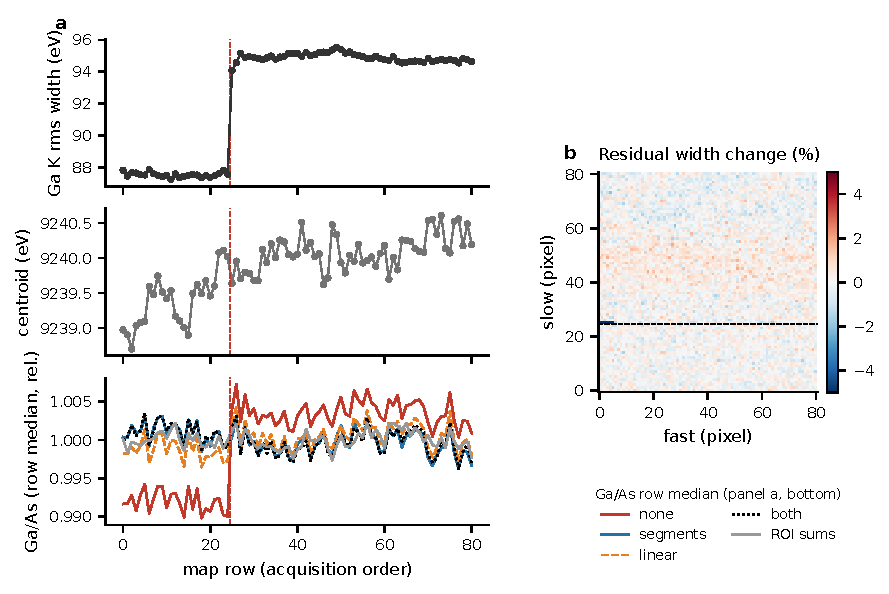
\includegraphics[width=\linewidth]{figures/fig08_resolution.pdf}
\caption{Resolution stability. (a) Per-row rms width and centroid of Ga~K$\alpha$ in acquisition
order, and row-median Ga/As area ratio for the four options of Table~\ref{tab:modes} and for plain
window sums (each normalised to its mean); the dashed line marks the detected step. (b) Residual
relative width change per pixel from the linear width term, with segments.}
\label{fig:resolution}
\end{figure}

%=====================================================================================
\section{Results on the (In,Ga)As film}\label{sec:results}
%=====================================================================================
\subsection{Maps}
Figure~\ref{fig:maps} shows the Ga~K and As~K areas and the Ga/As atom ratio of the film. The area maps
show the horizontal bands of the refills (Section~\ref{sec:refills}); the ratio map does not. The ratio
map has a median of \rxMed{} (\rxNoneMed{} without resolution tracking) and a pixel-to-pixel standard
deviation of \rxSpread. The statistical error expected from the area errors, scaled by the square root
of the median $\chi^2_\nu$, is \rxStat{} per pixel. The excess, $\sqrt{\rxSpread^2-\rxStat^2}=\rxExcess$
(\rxExcessNone{} without tracking), is real composition variation or residual systematics at the level
of half a per cent. Its pattern is not random: the ratio and the Ga map both show a diagonal
cross-hatch with a period of a few micrometres. Lattice-mismatched films often show such a
composition modulation along misfit-dislocation directions, and it can be compared directly with the
strain maps from the Laue patterns of the same scan.

\begin{figure}[t]
\centering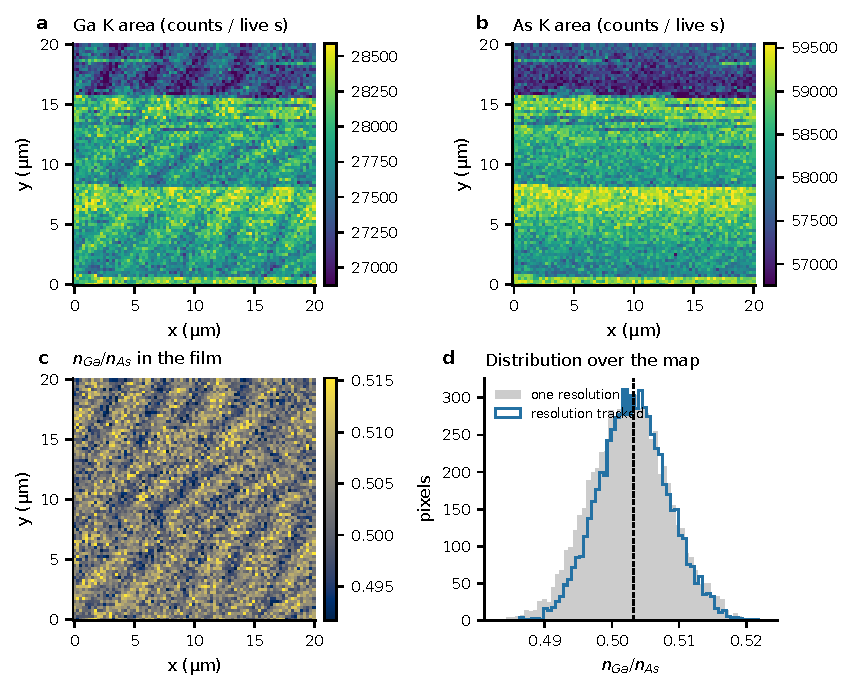
\includegraphics[width=\linewidth]{figures/fig09_maps.pdf}
\caption{Maps. (a, b) Ga~K and As~K group areas (all lines, per live second and unit relative monitor).
(c) Atom ratio $n_\mathrm{Ga}/n_\mathrm{As}$ in the (In,Ga)As film with resolution tracking (segments and
linear width term). (d) Distribution over the map with and without resolution tracking; the dashed line
is the median.}
\label{fig:maps}
\end{figure}

\subsection{Uncertainty budget}\label{sec:uncertainty}
The statistical error of the average is negligible. The accuracy is set by the model parameters that are
not measured. Table~\ref{tab:sensitivity} and Fig.~\ref{fig:sensitivity} requantify the same fitted areas
after changing one parameter at a time. The Ga/As ratio stays within \rxGaMin--\rxGaMax{}. The largest
effect is the air path (\qty{\pm2}{\percent} for \qty{\pm2}{cm}), because the efficiencies of Ga~K$\alpha$ and
As~K$\alpha$ are not equal; geometry, film thickness and pressure contribute a few tenths of a per cent.
The In content and the closure are a different matter: the closure ranges from \rClosureAirLo{} to
\rClosureAirHi{} for an air path of \num{18} to \qty{22}{cm}. Within an uncertainty of
\qty{\pm2}{cm} on the air path the measured closure is therefore not in contradiction with a
stoichiometric III/V film, but neither is it a measurement of the In content.

\begin{table}[t]
\centering
\caption{Sensitivity of the film composition to unmeasured parameters (same fitted areas,
requantified). Nominal: \qty{20}{cm} air at \qty{1013}{hPa}, $40^\circ$/$40^\circ$, film
\qty{1.9}{\micro\metre}, cap \qty{50}{nm}.}
\label{tab:sensitivity}
\begin{tabular}{lcccc}
\toprule
case & $n_\mathrm{Ga}/n_\mathrm{As}$ & change (\unit{\percent}) & $n_\mathrm{In}/n_\mathrm{As}$ & $(n_\mathrm{Ga}+n_\mathrm{In})/n_\mathrm{As}$\\
\midrule
\rSensitivityRows
\bottomrule
\end{tabular}
\end{table}

\begin{figure}[t]
\centering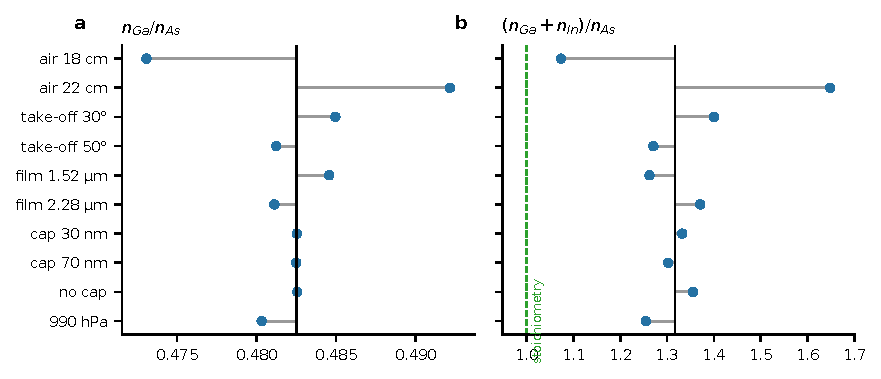
\includegraphics[width=\linewidth]{figures/fig10_sensitivity.pdf}
\caption{Sensitivity of (a) the Ga/As ratio and (b) the closure $(n_\mathrm{Ga}+n_\mathrm{In})/n_\mathrm{As}$
to the cases of Table~\ref{tab:sensitivity}; the vertical line is the nominal result and the dashed
line stoichiometry.}
\label{fig:sensitivity}
\end{figure}

%=====================================================================================
\section{Discussion and limitations}\label{sec:discussion}
%=====================================================================================
\paragraph{What is robust.} Ratios of lines of similar energy (Ga~K/As~K) are robust. Normalisation
cancels exactly, the beam spectrum enters only through the small difference between the Ga and As K
edges, and the detector and matrix corrections are similar for both lines. The two steps that make a
difference at the per-cent level are the bandwidth Jacobian (\qty{\rkJacobianBias}{\percent}) and the sample
model (\qty{\rMatrixEffect}{\percent}); resolution tracking matters at the level of \qty{1}{\percent} locally.

\paragraph{What is not.} Soft lines (In~L here, and generally L lines of $Z\lesssim55$ and K lines below
\qty{4}{keV}) depend exponentially on the sample--detector air path. The path is known to a few
centimetres only, and its effective length also depends on the take-off angle and on the beam position
on the sample. A one-centimetre error changes the In~L efficiency by \qty{\rInPerCmPct}{\percent}. The same
lines are the most absorbed in the sample and the most affected by the Neyman bias of the per-pixel solve.

\paragraph{Line shape.} The largest remaining misfit of the spectrum is the low-energy tail and shelf of
the strong lines. The fitted Lorentzian width (\qty{\rGamma}{eV}) partly mimics it. A tail that is not
modelled leaks into whatever lies just below a strong line: here Ga~K$\alpha$ into the Cu~K and Ni~K
region, and As~K$\alpha$ into Ga~K$\beta$.

\paragraph{Monitor.} The monitor over-responds at refills, which leaves \qty{2}{\percent} steps in all
absolute areas (Section~\ref{sec:refills}). Ratios are not affected.

\paragraph{Not addressed.} Laue Bragg reflections reaching the SDD would appear as narrow, position-dependent
peaks at arbitrary energies. None is obvious in the analysis region of this map, but the unidentified
\qty{15.8}{keV} peak may be one. Elastic and Compton scattering of the white beam is part of the
smooth background and is described by a polynomial, which is adequate over \qty{10}{keV} but not over
the full range. The incident spectrum is computed, not measured: mirror roughness, slope errors and the
exact air density are not constrained by the data, and they mainly affect the high-energy tail of the
band and the ratio of elements whose edges are far apart.

%=====================================================================================
\section{Recommendations}\label{sec:recommendations}
%=====================================================================================
\subsection{Instrument and acquisition}
\begin{enumerate}[leftmargin=*,itemsep=2pt]
\item \textbf{Measure the detection geometry for every experiment.} Record the sample--detector distance
(to $\pm\qty{2}{mm}$), the take-off angle and the incidence angle, and store them in the scan metadata.
Alternatively, flush the detection path with He or use a vacuum snout, which brings the In~L
efficiency from a few per cent to near unity and removes the dominant uncertainty of soft lines.
\item \textbf{Record the local pressure and temperature} (or take them from the ESRF logging), since
the In~L$\alpha$ efficiency through \qty{20}{cm} of air changes by \qty{\rLowPPct}{\percent} between \num{990} and \qty{1013}{hPa}.
\item \textbf{Characterise the monitor.} Measure its dark offset and linearity against the ring current,
or log the ring current with every point and model the monitor as $m=a+bI$; consider a monitor after
the KB mirrors.
\item \textbf{Fix and record the processor settings} (peaking time, gap, thresholds) and the detector
temperature for the whole scan; this would have avoided the resolution step of
Section~\ref{sec:resolution}.
\item \textbf{Extend the MCA range} to about \qty{30}{keV}. The upper part of the band excites the K lines
of In (\qty{24.2}{keV}) and the pile-up spectrum is fully recorded, which allows an independent In
quantification free of the air-path problem (but sensitive to the mirror cut-off).
\item \textbf{Keep the input rate moderate} (or use a shorter count time per point at lower rate) where
dead time exceeds \qtyrange{30}{40}{\percent}. Pile-up corrections are first order in the rate.
\end{enumerate}

\subsection{Calibration with standards}
\begin{enumerate}[leftmargin=*,itemsep=2pt,resume]
\item \textbf{Measure binary reference materials} in the same geometry: GaAs, InP and InAs wafers (bulk)
calibrate the Ga/As and In/As (and In/P) sensitivities directly, including the effective air path and
detector efficiency. A GaAs wafer would turn the closure test into a calibration of the In~L line.
\item \textbf{Measure a thin-film standard} (e.g.\ a certified multi-element thin film, or an In$_x$Ga$_{1-x}$As
layer of known $x$ and thickness from XRD or RBS) to test the thin-film matrix model separately from bulk
absorption.
\item \textbf{Validate the incident spectrum} with pure-element foils of increasing atomic number (e.g.\ Ti,
Cu, Zr, Ag, In, Sn): the K$\alpha$ yields of foils of known thickness map the spectral density across the band,
and a fit of the mirror angles, roughness and air path to them replaces the computed spectrum by a
measured one.
\end{enumerate}

\subsection{Analysis}
\begin{enumerate}[leftmargin=*,itemsep=2pt,resume]
\item \textbf{Fit the energy calibration} (gain and offset) on the average spectrum, or at least
check it against the strong lines, rather than holding the beamline calibration fixed.
\item \textbf{Add a low-energy tail and shelf} to the line shape (Hypermet-type step and exponential tail \citep{Phillips1976}, with amplitudes as smooth functions of energy). This is the largest remaining
misfit, and it biases peaks lying just below strong lines.
\item \textbf{Use model-based (Pearson) weights in the per-pixel solve}, $W_{cc}=s_i^2/\hat N_{ic}$, obtained by
one or two re-weighting iterations starting from Eq.~\eqref{eq:linear}, or a Poisson likelihood
\citep{Baker1984}; this removes the downward bias on weak peaks such as In~L.
\item \textbf{Treat Laue reflections explicitly}: detect narrow peaks that are not fluorescence lines from the
per-pixel residuals, and mask or model them pixel by pixel.
\item \textbf{Compute pile-up from the input rate} when the dead time is high, and allow the resolving
time to depend on the energies of the two pulses.
\item \textbf{Propagate the uncertainty budget}: report, with every map, the statistical error and the
systematic range from Table~\ref{tab:sensitivity}-type requantifications using the actual uncertainties of
geometry, air path and thicknesses.
\item \textbf{Use the closure as a consistency check, not as a constraint}. Fitting the air path to force
stoichiometry makes the In content agree by construction and hides any other error in the soft-line chain.
It is legitimate only once standards have shown that the remaining model is right.
\end{enumerate}

%=====================================================================================
\appendix
\section{Software}\label{sec:software}
%=====================================================================================
The chain is implemented in three modules at the root of the \code{pyXRT} repository; the notebook
\code{fluo\_analysis\_clean.ipynb} runs it with per-sample settings, and \code{make\_figures.py} in this
folder reproduces this document. Table~\ref{tab:software} maps the sections to the functions.

\begin{table}[h]
\centering\small
\caption{Where each step lives.}
\label{tab:software}
\begin{tabularx}{\linewidth}{>{\raggedright\arraybackslash}p{4.2cm}X}
\toprule
step & functions\\
\midrule
reading & \code{bliss\_hdf5\_reader.BlissMeshScan}\\
normalisation (Sec.~\ref{sec:norm}) & \code{xrf\_fit.normalise\_spectra}, \code{average\_spectrum}, \code{counting\_error}\\
incident beam (Sec.~\ref{sec:beam}) & \code{xrf\_beamline.BM32\_WHITE\_BEAM}, \code{Beamline.spectrum}, \code{per\_unit\_energy}\\
detector (Sec.~\ref{sec:detector}) & \code{xrf\_fit.Detector} (\code{from\_fwhm}, \code{sigma\_ev}, \code{efficiency}, \code{escape\_lines}),
\code{pileup\_spectra}, \code{average\_pileup\_template}\\
line groups (Sec.~\ref{sec:fp}) & \code{xrf\_fit.element\_line\_groups}\\
sample (Sec.~\ref{sec:matrix}) & \code{xrf\_matrix.Geometry}, \code{Layer}, \code{Stack}, \code{MatrixModel}\\
average fit (Sec.~\ref{sec:fit}) & \code{xrf\_fit.XRFModel}, \code{fit\_average\_spectrum}\\
quantification (Sec.~\ref{sec:quant}) & \code{xrf\_matrix.quantify\_layer}, \code{atom\_ratio}; \code{xrf\_fit.number\_ratio}\\
maps (Sec.~\ref{sec:maps}) & \code{xrf\_fit.fit\_map}, \code{MapResult}\\
resolution (Sec.~\ref{sec:resolution}) & \code{xrf\_fit.width\_window}, \code{peak\_width\_profile}, \code{detect\_steps},
\code{segment\_labels}, \code{fit\_segments}; \code{fit\_map(segments=, width\_correction=)}\\
\bottomrule
\end{tabularx}
\end{table}

\paragraph{Reproducing this document.} From the repository root, with \code{InPoSi\_v2\_center.h5} present:
\begin{verbatim}
python docs/xrf_quantification/make_figures.py  # figures, results.json (3 min)
python docs/xrf_quantification/make_macros.py   # results_macros.tex
cd docs/xrf_quantification && tectonic xrf_quantification.tex
\end{verbatim}
The first command runs the complete chain; the second turns its output into the \verb|\r...| macros used
for every number in the text.

\paragraph{Main settings.} Energy grid \qtyrange{3}{40}{keV} in \qty{10}{eV} steps; elements In, Ga, As, Cu,
Ni, Ca, Ar (K and L families); minimum relative line intensity \num{0.005}; analysis region
\qtyrange{2.9}{12.6}{keV}, background order 3; pile-up region \qtyrange{2.9}{20.3}{keV}, background
order 5; initial resolution \qty{135}{eV} at \qty{5.9}{keV} with $F=0.12$; secondary fluorescence on a
\qty{40}{eV} grid with 160 direction points; step detection window 5 rows, threshold 6, minimum
step \qty{1}{eV}.

\bibliographystyle{unsrtnat}
\bibliography{references}

\end{document}
